\documentclass[
	a4paper, 10pt,
	twocolumn
]{article}

\usepackage[utf8]{inputenc}
\usepackage[T2A]{fontenc}
\usepackage[english,russian]{babel}

\usepackage{tune}
\usepackage{lipsum}

\def\d{\,\mathrm{d}}
\def\div{\text{ --- }}

\begin{document}

%%% Title %%%

\begin{strip}
\begin{center}
\kern -2.4\baselineskip
{\bf\Large
	Глубоконеупругое рассеяние поляризованных электронов на нуклонах и спиновый кризис
}
\par\makeskip
{
	Керим Гусейнов\footnotemark
}
\par
{\it
	Московский государственный университет имени М.\,В.~Ломоносова, физический факультет, кафедра общей ядерной физики
}
\par
{
	\today
}
\end{center}
\end{strip}
\footnotetext{\href{mailto:guseynovkerim@gmail.com}{guseynovkerim@gmail.com}}

%%%%%%%%%%%%%%%%%%
%\begin{multicols}{2}
\section{Введение}

Протон -- самый легкий барион. Содержащиеся в нем три кварка должны находиться в наинизшем энергетическом состоянии. Логично ожидать, что волновая функция такой системы сферически симметрична, то есть орбитальный момент отсутствует. 

Поскольку, например, спин ядра в довольно успешной модели оболочек полностью описывается спинами нуклонов и не находится под влиянием переносчиков взаимодействия, мезонов, можно ожидать, что спин протона также определяется лишь кварками и не зависит от распределения глюонов. 
Исходя из этого, можно предположить, что два валентных кварка имеют сонаправленные спины, а третий противонаправлен им. 
Однако это рассуждение не подтверждается на эксперименте. 

Пользуясь современными представлениями о структуре адронов, необходимо перейти к партонным распределениям и структурным функциям. 
Сечение (в пределе скейлинга) глубоконеупругого рассеяния лептонов на адроне выражается через его партонные функции распределения $q_i(x)$ с помощью 
$$ F_1(x) = \frac{1}{2}\sum_i e_i^2 \, q_i(x), $$
$$ F_2(x) = \sum_i e_i^2 \, xq_i(x), $$
$$ \frac{\!\d^2\sigma}{\!\d\Omega\d E} = \frac{\alpha^2\,\cos^2(\theta/2)}{4\,E^2\,\sin^4(\theta/2)} \left( \frac{F_2}{\nu} + 2 \frac{F_1}{M}\,\tg^2(\theta/2) \right). $$

Для изучения спинов партонов необходимо разделить их распределения на два: с сонаправленным адрону спином и с противонаправленным. Тогда можно определить характеризующие спин структурные функции как 
\begin{equation*}
g_1(x) = \frac{1}{2} \sum_i e_i^2 \left( q_i^+(x) - q_i^-(x) \right),
\label{eq:g1.def}
\end{equation*}
$$ g_2(x) = \sum_i e_i^2\,x\left( q_i^+(x) - q_i^-(x) \right), $$
где `$+$' и `$-$' определяют знак проекции спина партона. 

Через поляризованные структурные функции выражается разность сечений поляризованных лептонов на поляризованных по и против лептонов адронах 
\begin{equation*}
\frac{\d\sigma^{\uparrow\uparrow} - \d\sigma^{\uparrow\downarrow}}
	{\d\sigma^{\uparrow\uparrow} + \d\sigma^{\uparrow\downarrow}} 
	\sim 
	\frac{g_1(x)}{F_1(x)}.
\label{eq:sigma.asym}
\end{equation*}

Упоминается лишь рассеяние лептонов, поскольку они являются точечными, и с помощью таких экспериментов можно достичь наибольшей точности измерений. 





\section{Обнаружение проблемы}
Правило сумм Бьеркена \cite{Bjorken1, Bjorken2} связывает интегралы $\int _0^1 g_1(x)\d x$ для протона и нейтрона и с поправками на эффекты излучения КХД \cite{Bj.fix1, Bj.fix2} имеет вид
\begin{equation}
\int\limits_0^1 \left(g_1^p(x) - g_1^n(x)\right)\d x = \frac{1}{6}\left|\frac{G_A}{G_V}\right|(1-\alpha_s/\pi).
\label{eq:gp-gn}
\end{equation}
Раздельные правила сумм для протона и нейтрона были выведены Эллисом и Яффе \cite{Ellis-Jaffe} в предположении нулевой поляризации странных кварков и, после поправок на КХД излучение \cite{E-J.fix}, интегралы принимают вид
\begin{equation}
\int\limits_0^1 g_1^p(x)\d x = \frac{1}{12}\left|\frac{G_A}{G_V}\right|\left(1+\frac{5}{3}\frac{3F/D - 1}{F/D + 1}\right) 
\label{eq:gp}
\end{equation}
для протона и 
\begin{equation}
\int\limits_0^1 g_1^n(x)\d x = \frac{1}{12}\left|\frac{G_A}{G_V}\right|\left(-1+\frac{5}{3}\frac{3F/D - 1}{F/D + 1}\right) 
\label{eq:gn}
\end{equation}
для нейтрона. В дальнейшем будем обозначать $\Gamma_{p,n} = \int_0^1 g_1^{p,n}\d x$.





%\section{Экспериментальное исследование}
Сама проблема была впервые обнаружена European Muon Collaboration в CERN \cite{MuonCollab}. В эксперименте рассеивались продольно поляризованные мюоны на содержащей водород мишени, состоящей из двух частей, поляризованных по и против поляризации мюонов. Измерения проводились в диапазонах $x = 0.01 \div 0.7$ и $Q^2 = 1.5 \div 70$~ГэВ$^2$.
Для условий эксперимента правила сумм дают $\Gamma_p = 0.189\pm0.005$, а сам эксперимент дал значительно меньшее значение $0.114\pm0.029$. Попробуем его проинтерпретировать. 

Вспомнив определение структурной функции $g_1$ и принимая во внимание лишь валентные кварки, запишем 
$$ 
g^p_1(x) = \frac{1}{2}\left(
	\frac{4}{9}\left(u^+-u^-\right) + 
	\frac{1}{9}\left(d^+-d^-\right)
\right).
$$
Спин протона $S_z$ в таком случае выражается как
$$
S_z = \frac{1}{2} = 
\int\limits_0^1 \left(
	\frac{1}{2}u^+ - \frac{1}{2}u^- +
	\frac{1}{2}d^+ - \frac{1}{2}d^-
\right)\!\!\d x.
$$
Обозначим $\Delta q \equiv \int_0^1(q^+-q^-)\d x$. Тогда $S_z = \frac{1}{2}\Delta u + \frac{1}{2}\Delta d$, $\Gamma_p = \frac{4}{18}\Delta u + \frac{1}{18}\Delta d$. Единственной структурной функцией протона не обойтись, поэтому, предположим справедливость правила сумм Бьеркена. Поскольку $\Gamma_n = \frac{1}{18}\Delta u + \frac{4}{18}\Delta d$ и в условиях эксперимента
\begin{equation*}
\Gamma_p - \Gamma_n = \frac{\Delta u - \Delta d}{6} = 0.191 \pm 0.002,
\end{equation*}
получаем $\Delta u = 0.64\pm0.10$, $\Delta d = -0.51\pm0.10$ и 
$$
S_z = \frac{\Delta u + \Delta d}{2} = 0.07 \pm 0.10.
$$
Это значит, что при таком простом рассмотрении спин протона вообще не содержит вклада кварков. 
Анализ показывает \cite{EMC.theory.fix}, что даже при более детальном рассмотрении с учетом высших поправок КХД, переносимый валентными кварками спин пренебрежимо мал. 

В попытках понять, что же дает протону его спин, можно обратиться к морским кваркам, дикваркам и орбитальному моменту партонов. Можно также засомневаться в правиле сумм Бьеркена, но это наименее предпочтительно, поскольку оно выводилось лишь в предположении изоспиновой симметрии. 

Морские кварки, по определению, это те, для которых $ q_\mathrm{sea}(x) = \bar{q}_\mathrm{sea}(x) $. Исходя из этого равенства и изоспиновой симметрии выходит, что морские $u$- и $d$-кварки не влияют на спин протона. Тогда с учетом вкладов глюонов $\Delta g$ и морских странных кварков
\begin{equation*}
S_z = S_z^\mathrm{val} + \frac{3}{5}\Delta s + \Delta g.
\end{equation*}
Из асимптотической свободы следует, что полный переносимый кварком спин не должен зависеть от $Q^2$ \cite{AltarelliParisi}. Поэтому, если в имеющемся эксперименте вклад морских странных кварков велик, то он должен быть велик и во всех других сценариях, что, вероятно, может привести к проблемам при описании других статичных свойств адронов. 
Спин, переносимый глюонами, в свою очередь, зависит от $Q^2$, но только логарифмически, поэтому может быть большим в эксперименте EMC только, если он по какой-то загадочной причине велик изначально.

Касательно дикварков в протоне нужно сказать, что при больших переданных импульсах их влияние не может быть существенным, поскольку кварки испытывают асимптотическую свободу. Однако при $Q^2 < 10$ ГэВ$^2$ может, поэтому необходима какая-то оценка. Если принять во внимание $(uu)$ и $(ud)$ дикварки и выбрать какое-то похожее на разумное их распределение по продольным долям импульса, окажется, что для значимого вклада в спин протона вероятность их образования должна быть неправдоподобно большой. Значит, дикварки маловероятно переносят ненулевую долю спина. 

В принципе, ничего не запрещает спину адронов происходить от углового момента. Даже используя примитивную оценку 
$$L \lesssim \langle p_T \rangle R, $$
где $R$ -- радиус адрона, а $\langle p_T \rangle$ -- средний поперечный импульс партонов, для $R=1$~фм, $\langle p_T \rangle \sim 0.2$~ГэВ получаем $L \lesssim 1$, что не запрещает $\langle L_z \rangle$ быть вблизи $1/2$. Непонятно, однако, почему основное состояние трехкварковой системы, протон, обладает существенно ненулевым орбитальным моментом, и как это будет отражаться на других характеристиках нуклонов. 

Стоит заметить, что в хиральных моделях ($m_q~\!\!=~\!\!0$) спин протона содержит тождественно равный нулю вклад спинов кварков и складывается лишь из спинов глюонов и орбитальных моментов всех партонов \cite{Chiral}. 

В итоге на первых этапах изучения проблемы можно заключить, что спин протона происходит от глюонов и орбитального движения партонов. 

Более точные эксперименты были проведены E143 Collaboration \cite{E143} на SLAC и COMPASS Collaboration в CERN \cite{COMPASS}. Их результаты показали, что валентными кварками переносится треть спина протона, а само значение $\Gamma_p$ составляет $0.132\pm0.010$.


\section{Структурная функция нейтрона}
В свете всего сказанного, важной представляется прямая экспериментальная проверка правила сумм Бьеркена. Для ее осуществления необходимо определить структурную функцию нейтрона $g_1^n$ в достаточно широком диапазоне $x$, особенно важна область малых значений. 
Так как нейтроны в свободном состоянии распадаются и создать чисто нейтронную мишень не представляется возможным, необходимо использовать какое-то ядро. 
На первый взгляд может показаться, что идеальной мишенью будут дейтроны, однако необходимо учесть, что в дейтронах спин нейтрона складывается со спином протона и, естественно, образует состояние с определенным значением суммы спинов. В таких состояниях складывающиеся спины абсолютно неполяризованы. Это значит, что в дейтроне принципиально не определено направление спина нейтрона, и такая мишень не подходит для анализа.

Очень хорошим вариантом оказывается мишень из $^3$He, поскольку ядра состоят из двух спаренных, а значит находящихся в синглетном спиновом состоянии, протонов и нейтрона без орбитального момента. Спин нейтрона ни с чем не взаимодействует, и поэтому спиновая асимметрия $^3$He будет максимально близка к асимметрии в нейтроне. 
Эксперименты с такой мишенью были проведены E154 Collaboration \cite{E154} и E155 Collaboration \cite{E155} на SLAC. В них использовались поляризованные электроны, рожденные с помощью лазерной фотоэмиссии и затем разогнанные. Циклическая смена поляризации пучка и мишени позволила существенно уменьшить систематические погрешности. Диапазоны динамических переменных составляли $x = 0.014 \div 0.8 $ и $Q^2 = 1 \div 40 $~ГэВ$^2$. 

Поскольку экспериментально измерить структурные функции во всем диапазоне от $0$ до $1$ невозможно, необходимо использовать какие-то модельные зависимости $g_1(x)$ при малых $x$. Аппроксимируя отрицательной степенной зависимостью, можно получить результат $\Gamma_n = -0.041\pm0.007$. К сожалению, это число не оказывается пренебрежимо мало зависящим от выбора модели.

Из приведенных результатов видно, что правило сумм Бьеркена не нарушается: $\Gamma_p - \Gamma_n = 0.173 \pm 0.012$ из эксперимента и $ 0.182\pm0.005 $ из теории при соответствующем $Q^2=5$~ГэВ$^2$. 



\section{Морские кварки}
Для определения индивидуальных вкладов различных типов кварков необходимо отказаться от полностью инклюзивных процессов и регистрировать какие-то адроны, преимущественно мезоны, вылетающие из протона после рассеяния. 
Такие полуинклюзивные измерения с регистрацией пионов и каонов были проведены HERMES Collaboration \cite{HERMES} и COMPASS Collaboration \cite{COMPASS.sea}. 
Для морских странных кварков данные HERMES показали $\int_{0.02}^{0.6}\Delta s\d x = 0.037 \pm 0.033$, а COMPASS -- $\int_{0.004}^1 \Delta s \d x = -0.02 \pm 0.04$, что полностью согласуется с нулевым вкладом странного моря. 
Влияние морских $\bar{u}$ и $\bar{d}$ кварков также изучалось в этих экспериментах, оно оказалось тоже нулевым. Экспериментальные данные по морским кваркам ничуть не противоречат первым теоретическим анализам происхождения спина протона: он не находится под влиянием кваркового моря. 

\section{Поляризация глюонов}
\begin{figure}
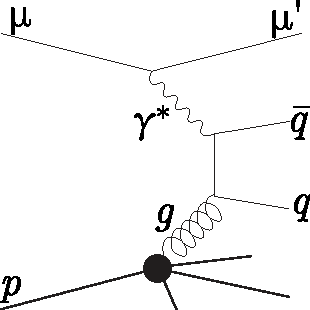
\includegraphics[width=.6\linewidth]{figs/Gluon-g1}
\caption{Образование кварк-антикварковой пары при взаимодействии виртуального фотона с глюоном.}
\label{fig:gluon}
\end{figure}

Очевидно, рассеяние поляризованных протонов на поляризованных протонах чувствительно к распределению глюонов и их спинов, однако при изучении таких процессов, помимо сложности выделения и восстановления нужного сигнала, возникает еще и дополнительная ошибка, связанная с тем, что обе взаимодействующие частицы не являются точечными. 
COMPASS Collaboration впервые предложила так называемое глюон-фотонное слияние, при котором виртуальный фотон и глюон взаимодействуют, превращаясь в кварк-антикварковые пары, и в результате образуют кварк-антикварковую пару. Этот процесс изображен на Рис. \ref{fig:gluon}.
Его сечение в первом Борновском приближении прямо пропорционально поляризованным функциям распределения глюонов. Поскольку три легких кварка рождаются слишком часто, выделить нужные события можно по рождению $c$-кварка и очарованных мезонов. 
Однако эксперименты COMPASS Collaboration нельзя считать подтверждением ненулевого вклада глюонов в спин протона \cite{COMPASS.gluon1, COMPASS.gluon2}. 

Многие другие эксперименты по определению $\Delta g$ не принесли большого успеха и не смогли подтвердить или опровергнуть какую-либо теорию \cite{HERMES.gluon,STAR.gluon,PHENIX.gluon}.


\section{Выводы}
Вызов понять внутреннюю структуру спина протона вдохновил научное сообщество на невероятно большую теоретическую и экспериментальную работу на протяжении всех лет с момента обнаружения проблемы. Касательно продольной структуры спина было достигнуто согласие между экспериментальными данными разных групп, если принять во внимание эволюцию с $Q^2$ и кинематические особенности каждого эксперимента. Теоретическое описание соответствующих величин также пришло к согласию с данными.

Полуинклюзивные измерения показали отсутствие значимого вклада морских кварков, включая странный, в спин протона, и полный вклад спинов кварков по современным представлениям составляет $\Delta u + \Delta d \approx 0.35$. Основные модели, описывающие столь малое значение, подразумевают перенос спина валентных кварков в орбитальное движение из-за пионных облаков. Спиный кризис должен что-то говорить о взаимодействии валентных кварков, хиральной динамики и сложной структуры вакуума квантовой хромодинамики. Будущие эксперименты нацелены в основном на уточнение вкладов глюонной поляризации и странного моря. 

Кроме того, ожидается все же ненулевой орбитальный момент валентных кварков, как минимум из-за конфайнмента, для которого необходим поперечный масштаб. Большой интерес представляет и спин-орбитальное взаимодействие в КХД, поскольку оно может объяснить большие поперечные асимметрии в рассеянии. Достижение понимания и измерение орбитальных моментов в КХД пробудило дополнительный интерес к изучению трехмерной структуры нуклонов.

Необходимость изучения поперечной структуры нуклона приводит и к большой теоретической работе по построению моделей в областях, где важны эти размеры, численному расчету вкладов глюонов и странного моря и извлечению новых характеристик нуклона из измеряемых в эксперименте величин. 







\bibliographystyle{local}
\bibliography{Refs}
\end{document}



%\end{multicols}


\clearpage
%\begin{multicols}{2}
\appendix
\section{Переменные глубоконеупругого рассеяния}
$$ y = \frac{q \cdot p}{k \cdot p} $$
$$ Q^2 = -q^2 $$
$$ x = \frac{Q^2}{2\, p \cdot q} $$
%\end{multicols}


\end{document}
